\chapter{Personalplaner}\label{personal:mitglieder}
Im Kopf des Fensters aus \cref{fig:personal:mitglieder} kann eingestellt werden welche Personen angezeigt werden sollen.
Ebenso kann durch einen Knopfdruck eine E-Mail an alle angezeigten Personen erstellt werden.
Werden bei dieser Aktion Personen gefunden, für die keine Mailadresse angegeben ist,
so können die angegebenen Postadressen in einer CSV-Datei gespeichert werden.
Diese Daten können dann z.B.\ für Serienbriefe genutzt werden.


\begin{figure}[!h]
	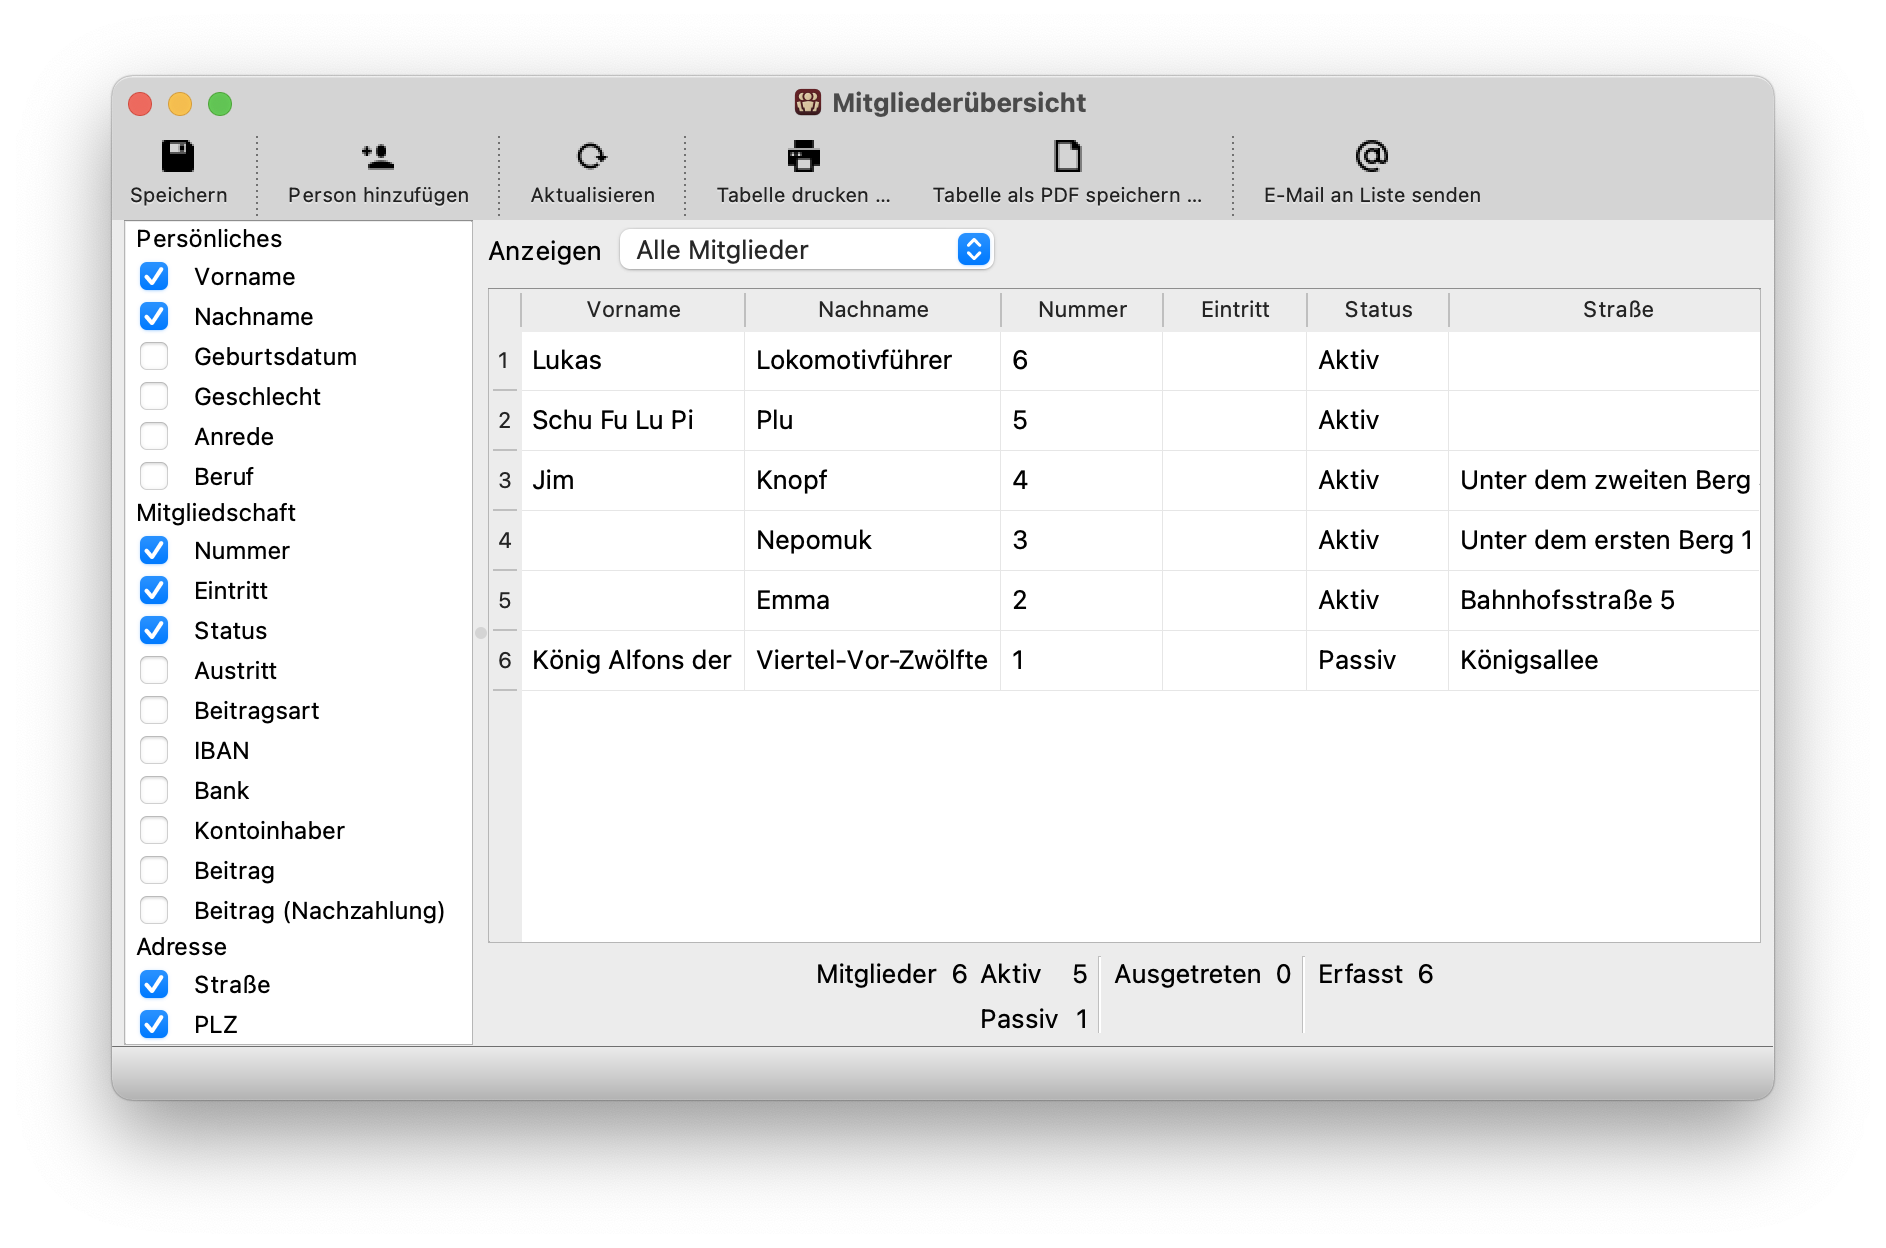
\includegraphics[width=\textwidth]{img/personal-liste}
	\caption{Die Mitgliederliste mit allen ausgewählten Mitgliedern.}
	\label{fig:personal:mitglieder}
\end{figure}

In der Tabelle werden alle gespeicherten Daten der ausgewählten Mitglieder angezeigt.
Diese Tabelle kann über das Menü \aktion{Exportieren} unter dem Punkt \aktion{Mitgliederliste} ausgegeben werden.
Ebenso stehen hierzu die Knöpfe \button{Tabelle drucken} und \button{Tabelle als PDF speichern} ausgegeben werden.
Über das Menü ist darüber hinaus noch eine Ausgabe als CSV-Datei möglich,
sodass die Daten in anderen Programmen verarbeitet werden können.
Ebenso besteht die Möglichkeit über den Eintrag \aktion{Stammdatenblätter} die Daten eines Mitglieds bzw.\ aller angezeigten Personen auszugeben.
Hierbei wird für jede Person eine Seite erzeugt und kann somit auch für jede Person getrennt gespeichert werden.

Darüber hinaus wird im unteren Bereich des Fensters eine kurze Statistik
der aktuellen und ausgetretenen Mitglieder angezeigt.
